\chapter{Wazuh Agent Installation}

\section{Installation via GPO}
Der Wazuh Agent kann per Group Policy auf allen Windows Geräten installiert werden.
Dazu muss als erstes die Installationsdatei für den Agent auf der \href{https://documentation.wazuh.com/current/installation-guide/packages-list.html}{Webseite von Wazuh}\footnote{Link: https://documentation.wazuh.com/current/installation-guide/packages-list.html} heruntergeladen werden.\\

Die Installationsdatei braucht eine Konfigurationsdatei welche die Netzwerkadresse des Wazuh Managers enthält.
Eine solche Konfigurationsdatei kann mithilfe dem Windows Tool ``Orca'' erstellt werden, welches Teil der Windows SDK ist. Das Windows SDK kann man auf der \href{https://developer.microsoft.com/de-de/windows/downloads/windows-sdk/}{Webseite von Microsoft}\footnote{Link: https://developer.microsoft.com/de-de/windows/downloads/windows-sdk/} herunterladen.\\

Bei der Installation der Windows SDK kann eine grosse Anzahl Features ausgewählt werden.
Für Orca wird jedoch nur das Feature ``MSI Tools'' benötigt, alle andere Features können abgewählt werden.
\begin{figure}[H]
    \centering
    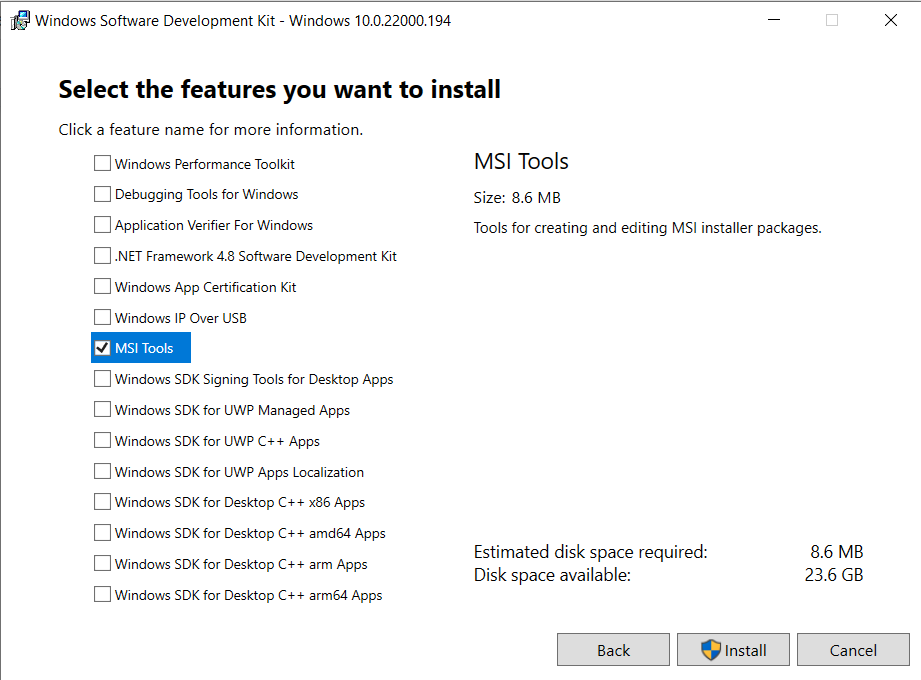
\includegraphics[width=0.7\linewidth]{../img/agent/install-sdk.png}
    \caption{MSI Tools der Windows SDK}
\end{figure}

Orca befindet sich nun unter
\begin{lstlisting}
    C:\Program Files (x86)\Windows Kits\10\bin\<Version>\x86\Orca-x86_de-de.msi
\end{lstlisting}
und kann mit dieser .msi Installationsdatei installiert werden.
Sobald Orca installiert ist wird im Kontextmenu bei .msi Dateien einen neuen Punkt mit ``Edit with Orca'' ersichtlich.\\

Mit einem Rechtsklick auf die Wazuh Agent .msi Datei kann via ``Edit with Orca'' eine Konfigurationsdatei erstellt werden.
\begin{figure}[H]
    \centering
    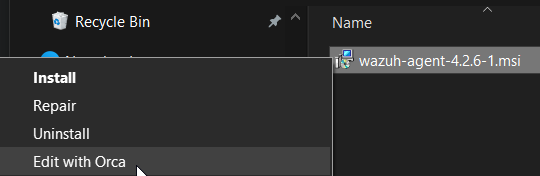
\includegraphics[width=0.7\linewidth]{../img/agent/edit-with-orca.png}
    \caption{Mit Orca bearbeiten}
\end{figure}

In Orca muss man in der Menüleiste unter \textbf{Transform $\rightarrow$ New Transform} einen neuen Änderungsnachweis erstellen.
\begin{figure}[H]
    \centering
    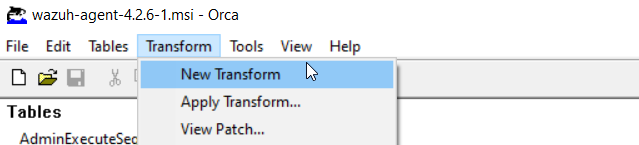
\includegraphics[width=0.7\linewidth]{../img/agent/new-transform.png}
    \caption{Neuer Änderungsnachweis in Orca}
\end{figure}

Auf der linken Seite unter ``Tables'' auf die Tabelle ``Property'' gehen.
Dort werden neue ``Key - Value'' Paare hinzugefügt.
Es braucht folgende Paare:
\begin{itemize}
    \item \textbf{WAZUH\_MANAGER}: <Hostname Wazuh Manager>
    \item \textbf{WAZUH\_REGISTRATION\_SERVER}: <Hostname Wazuh Manager>
    \item \textbf{WAZUH\_AGENT\_GROUP}: Windows
    \item \textbf{WAZUH\_REGISTRATION\_PASSWORD}: <Password gesetzt bei Installation>
\end{itemize}

\begin{figure}[H]
    \centering
    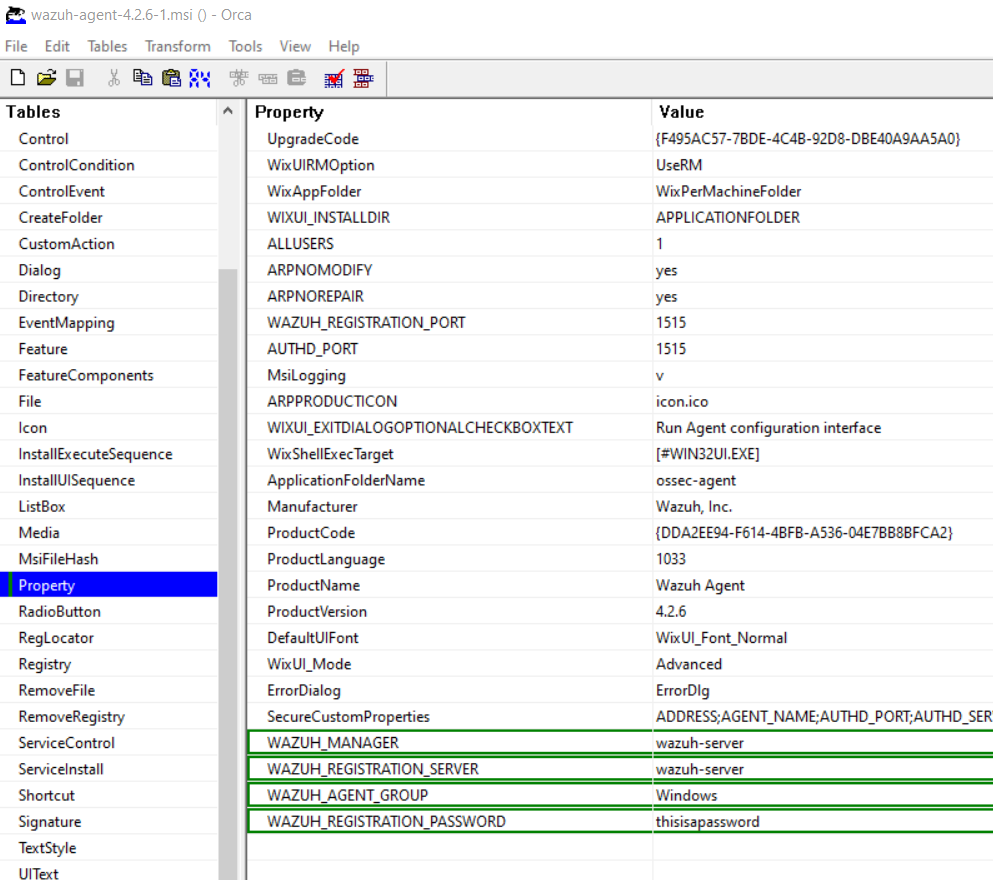
\includegraphics[width=0.7\linewidth]{../img/agent/Orca-Edit.png}
    \caption{Wazuh Installationsparameter}
\end{figure}

In der Menüleiste unter \textbf{Transform $\rightarrow$ Generate Transform} die Konfigurationsdatei exportieren und unter einem beliebigen Namen, zum Beispiel ``custom-wazuh-settings.mst'', abgespeichern.\\

Die .msi und .mst Dateien müssen nun in einem freigegebenen Netzlaufwerk abgespeichert werden, auf welches alle Windows Geräte Zugriff haben. Zum Beispiel auf dem Domain Controller unter:
\begin{lstlisting}
    C:\Windows\SYSVOL\sysvol\<Domain>
\end{lstlisting}

Nun muss eine neue Group Policy erstellt werden, mit welcher der Wazuh Agent auf den Windows Geräten installiert wird.
Dazu öffnet man das Group Policy Management auf dem Domain Controller und erstellt eine neue Group Policy, welche mit der OU verknüpft ist, die alle Windows Geräte enthält.
\begin{figure}[H]
    \centering
    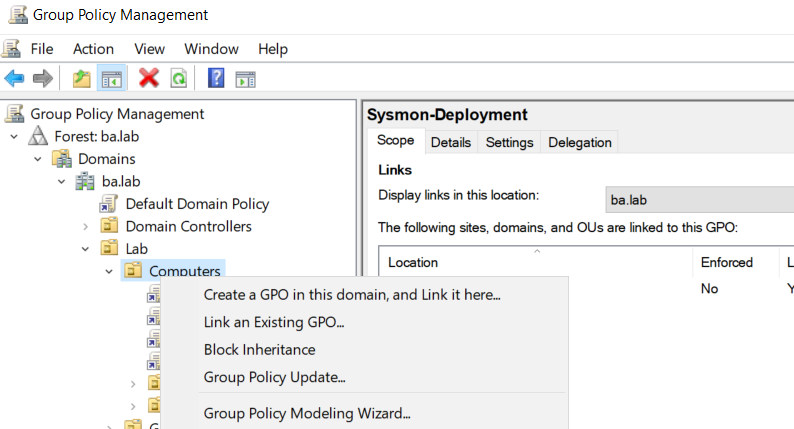
\includegraphics[width=0.7\linewidth]{../img/agent/create-new-group-policy.png}
    \caption{Neue Group Policy für Agent Deployment}
\end{figure}

In der neuen Group Policy muss unter \textbf{Computer Configuration $\rightarrow$ Policies $\rightarrow$ Software Settings $\rightarrow$ Software installation} mit \textbf{Rechtsklick $\rightarrow$ New $\rightarrow$ Package\dots} eine Datei ausgewählt werden, welche installiert werden soll.

\begin{figure}[H]
    \centering
    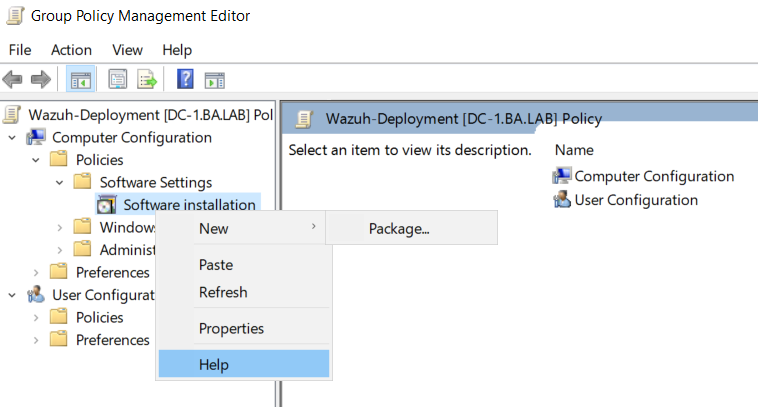
\includegraphics[width=0.7\linewidth]{../img/agent/new-software-install.png}
    \caption{Neue Group Policy für Agent Deployment}
\end{figure}
Im neuen Fesnter wählt man die .msi Datei, welche im freigegebenen Netzlaufwerk abgelegt wurde.
Beim Installationstyp wählt man anschliessen ``Advanced'' und klickt weiter.
Ein neues Fenster öffnet sich, in welchem man Anpassungen für die Installation angeben kann.
Unter \textbf{Modifications $\rightarrow$} wählt man nun die .mst Datei aus, welche vorher erstellt wurde.\\

Nun kann man mit OK Bestätigen.
Die Group Policy ist bereit und kann geschlossen werden.
Der Wazuh Agent wird beim Einloggen auf den Geräten installiert und verbindet sich automatisch mit dem Server.


\section{Manuelle Installation}

Der Wazuh Agent kann über die Commandline von mehreren Betriebssystemen installiert werden.
Für Windows zum Beispiel mit Powershell.
Die Commands der einzelen Betriebssystem findet man im Wazuh Manager.
Dazu öffnet man den Wazuh Manager und geht auf \textbf{Wazuh $\rightarrow$ Agent}.
Auf der rechten Seite der Tabelle mit allen Agents klickt man auf ``Deploy new Agent''.
\begin{figure}[H]
    \centering
    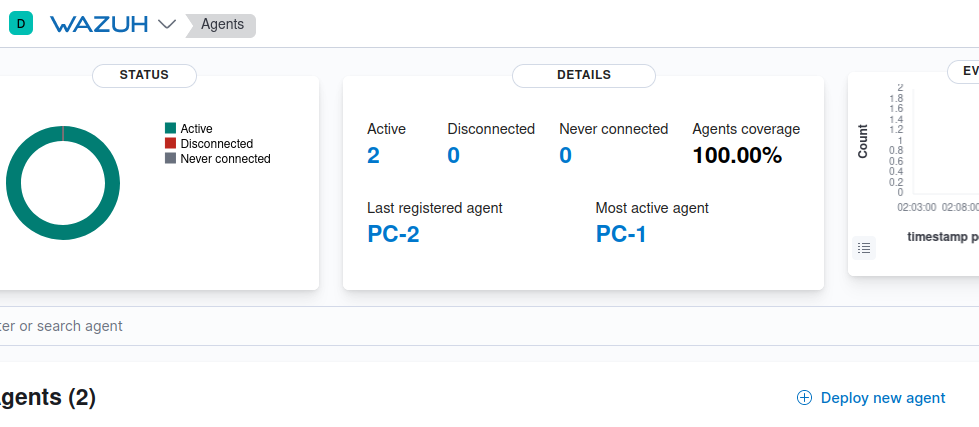
\includegraphics[width=0.7\linewidth]{../img/agent/deploy-new-agent.png}
    \caption{Agent deployment}
\end{figure}

Auf der nächsten Seite gibt man alle nötigen Daten an und kann unten den Powershell Command kopieren.
\begin{figure}[H]
    \centering
    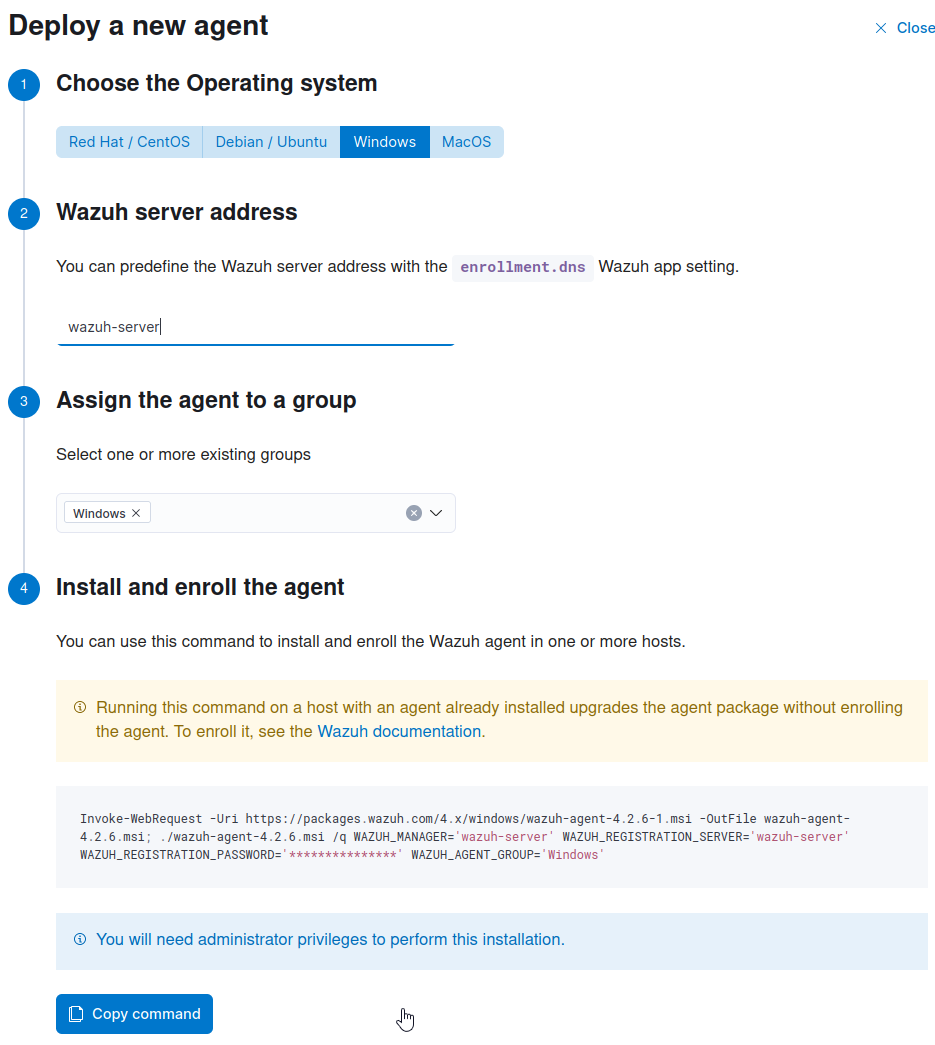
\includegraphics[width=0.7\linewidth]{../img/agent/deploy-new-agent-2.png}
    \caption{Wazuh Agent manuell installieren}
\end{figure}

Auf dem Windows Gerät Powershell als Administrator starten und das zuvor kopierte Command eingeben:

\begin{lstlisting}
    Invoke-WebRequest -Uri https://packages.wazuh.com/4.x/Der Wazuh/wazuh-agent-mit einem.2.6-1.msi -OutFile wazuh-agent-4.2.6.msi; ./wazuh-agent-4.2.6.msi /q WAZUH_MANAGER='wazuh-server' WAZUH_REGISTRATION_SERVER='wazuh-server' WAZUH_REGISTRATION_PASSWORD=<Password> WAZUH_AGENT_GROUP='Windows' 
\end{lstlisting}

Auf der Deployment Seite vom Wazuh Manager können auch Red Hat, Debian und MacOS ausgewählt werden.
Dann werden die Commands für diese Geräte angezeigt.